\documentclass[12pt]{extreport}

\usepackage{amsmath, amsthm, amssymb, amsfonts, mathtext}
\usepackage[T1,T2A]{fontenc}
\usepackage[utf8]{inputenc}
\usepackage[english, russian]{babel}
\usepackage[babel=true]{microtype}
\usepackage{float}

\usepackage{caption, subcaption}
\captionsetup[table]{
	position=top,
	justification=raggedleft,
	singlelinecheck=false,
	aboveskip=0pt
}


\usepackage{geometry, graphicx, wrapfig, flafter, multirow, booktabs, derivative}

\graphicspath{{images/}}

\geometry{top=2cm, bottom=2cm, left=2cm, right=1cm}

\usepackage{fancyhdr}

\usepackage{listings}
\lstset{language=C++}

\let\oldcaptionbox\captionbox
\renewcommand{\captionbox}[2]{%
	\refstepcounter{table}%       <-- принудительно увеличиваем счётчик таблицы
	\addtocounter{table}{-1}% 
	\oldcaptionbox{#1}{#2 \label{}}% <-- оставляем пустую метку внутри
	
	
}



\begin{document}
	\begin{titlepage}
		\begin{center}
			{\small МИНИСТЕРСТВО НАУКИ И ВЫСШЕГО ОБРАЗОВАНИЯ РОССИЙСКОЙ ФЕДЕРАЦИИ \\
				ФЕДЕРАЛЬНОЕ ГОСУДАРСТВЕННОЕ АВТОНОМНОЕ ОБРАЗОВАТЕЛЬНОЕ УЧРЕЖДЕНИЕ ВЫСШЕГО ОБРАЗОВАНИЯ \\
				<<МОСКОВСКИЙ ФИЗИКО-ТЕХНИЧЕСКИЙ ИНСТИТУТ \\
				(НАЦИОНАЛЬНЫЙ ИССЛЕДОВАТЕЛЬСКИЙ УНИВЕРСИТЕТ)>>\\
				Кафедра общей физики}
			
			\vfill
			
			{\large \textbf{Вопрос по выбору}}\\
			
			\vspace{0.5cm}
			
			{\Large\textbf{Измерение показателя адиабаты воздуха}} \\
			{\Large\textbf{по температурной зависимости частоты}} \\
			{\Large\textbf{резонатора Гельмгольца}}	
			
			\vfill
			
			\begin{flushright}
				\begin{tabular}{r l}
					Выполнили: & студент группы Б04-507 Рудачихин П.А. \\
					& студент группы Б04-507 Свиногонов М.А. \\	
				\end{tabular}
			\end{flushright}
			\vfill
			Москва \\
			2026 г.
		\end{center}
	\end{titlepage}
	
	
	\pagestyle{empty}
	\tableofcontents
	\clearpage
	\pagestyle{fancy}	
	\fancyhf{}
	\fancyhead[L]{\leftmark}
	\fancyhead[R]{\rightmark}
	\fancyfoot[C]{\thepage}
	
	\chapter{Введение}
	
	\section{Аннотация}
	
	\hspace{4mm} В данном вопросе по выбору рассмотрен экспериментальный способ определения показателя адиабаты (отношения теплоёмкостей) воздуха с помощью стеклянной банки, используемой как резонатор Гельмгольца. Его частота собственного резонанса определяется скоростью звука в воздухе, которая зависит от показателя адиабаты. 
	
	Для того чтобы корректно перейти от измеренной частоты к величине \(\gamma\), необходимо учитывать не просто геометрическую длину горлышка резонатора, а эффективную длину. Поэтому эксперимент состоит из двух этапов: сначала определяется эффективная длина горлышка методом добавочных шеек, затем снимается температурная зависимость частоты резонанса.
	
	Исследование охватывает несколько разделов курса общей физики: термодинамика, молекулярная физика, акустика, колебания и экспериментальные методы обработки данных.
	
	Эта тема представляется удачной по нескольким причинам:
	\begin{itemize}
		
		\item определение показателя адиабаты воздуха --- содержательная термодинамическая цель;
		\item результат эксперимента легко верифицируем: значение показателя адиабаты приведено в справочной литературе с высокой точностью;
		\item в эксперименте реализуется и исследуется физическая модель --- резонатор Гельмгольца;
		\item методика эксперимента комплексная, так как включает две независимых серии измерений;
		\item работа имеет практическое значение, так как включает разработку экспериментальной установки и методики измерения.
		
	\end{itemize}
	
	\section{Цель работы}
	
	\hspace{4mm} Целью данного вопроса по выбору является \textit{разработка и теоретическое обоснование метода экспериментального определения показателя адиабаты по температурной зависимости частоты основного резонанса банки, рассматриваемой как резонатор Гельмгольца, с предварительным определением эффективной длины горлышка методом добавочных шеек.}
	
	
	\section{Используемые материалы и оборудование}
	
	\hspace{4mm} Для создания экспериментальной установки мы использовали следующие \textbf{материалы}:
	\begin{enumerate}
		\item стеклянную банку;
		\item специальную крышку: соединённые металлическая и пластмассовая крышки со слоем пенопласта между ними с отверстиями для добавочных трубок и проводов наушников;
		\item герметик для устранения течей;
		\item набор цилиндрических пластиковых трубок одного внутреннего диаметра и разной длины;
		\item алюминиевую фольгу для теплоизоляции;
		\item груз-балласт для погружения резонатора;
		\item изоленту и скотч.
	\end{enumerate}
	
	Для проведения эксперимента мы использовали следующий набор \textbf{оборудования}:
	\begin{enumerate}
		\item штангенциркуль с ценой деления нониуса 0,05 мм для измерения диаметра и длины трубок;
		\item цифровые весы MH-500 с дискретностью 0,1 грамм для измерения массы банки и заполняющей её воды;
		\item проводные наушники для возбуждения и регистрации акустических колебаний;
		\item термостат ЛОИП LT-100 с точностью поддержания температуры 0,1 $^oС$ для изменения и поддержания температуры воздуха в банке;
		\item цифровой датчик температуры DS18B20 и два термощупа TP101 для контроля температуры воздуха на разных уровнях внутри банки.
	\end{enumerate}		
	
	В работе использовался компьютер со следующим \textbf{программным обеспечением}:
	
	\begin{enumerate}
		
		\item <<REW>> для генерации звукового сигнала и спектрального анализа;
		\item <<MS Excel>> и <<OriginPro>> для обработки данных и построения графиков.
	\end{enumerate}	
	
	
	
	\chapter{Теоретические сведения}
	
	\hspace{4mm} Одной из важных характеристик газа является его показатель адиабаты 
	\[
	\gamma=\frac{C_P}{C_V},
	\]
	
	где $C_P$ --- теплоёмкость при постоянном давлении,  $C_V$ --- при постоянном объёме.
	
	
	Существует несколько способов  его определения, один из которых основан на измерении скорости звука. 
	
	
	В газе звуковые колебания протекают настолько быстро, что теплообменом между областями сжатия и разрежения можно пренебречь. Поэтому звуковой процесс адиабатический, и скорость звука зависит от \(\gamma\).
	
	
	Если использовать в качестве акустической системы резонатор Гельмгольца, то связь со скоростью звука становится особенно удобной: от неё зависит частота основного резонанса. Измеряя эту частоту в зависимости от температуры, можно определить \(\gamma\).
	
	
	\section{Резонатор Гельмгольца}
	
	\begin{wrapfigure}[18]{r}{0.25\textwidth}
		\centering
		
\includegraphics[width=\linewidth]{resonator_scheme}
		\caption{Схема резонатора Гельмгольца.}
		\label{fig:resonator}
	\end{wrapfigure}
	
	
	\hspace{4mm} Рассмотрим \textit{резонатор Гельмгольца}, состоящий из полости объёма \(V\) и узкой шейки с площадью поперечного сечения \(S\). Пусть эффективная длина шейки равна \(L_{\text{эфф}}\). Тогда воздух, находящийся в шейке, можно рассматривать как своеобразную \textit{воздушную пробку}, которая движется вдоль оси шейки как единое целое.
	
	Пусть эта воздушная пробка сместилась внутрь или наружу на малую величину \(x\). Тогда объём воздуха в основной полости изменится на величину
	
	\begin{equation}
		\Delta V = Sx.
		\label{eq:dV}
	\end{equation}
	
	Поскольку акустические колебания происходят достаточно быстро, процесс сжатия и разрежения воздуха в резонаторе можно считать адиабатическим. Для адиабатического процесса идеального газа выполняется условие
	
	
	\begin{equation}
		pV^\gamma=\mathrm{const},
		\label{eq:adiab}
	\end{equation}
	
	
	где \(p\) --- давление воздуха в полости, \(V\) --- объём полости.
	
	Рассмотрим малое отклонение от равновесия. Продифференцируем \eqref{eq:adiab}:

	
	\begin{equation}
		d(pV^\gamma)=0 \Rightarrow V^\gamma\,dp+\gamma pV^{\gamma-1}\,dV=0 \Rightarrow  dp=-\gamma p\frac{dV}{V}
		\label{eq:dp}
	\end{equation}
	
	
	Для малых колебаний вместо дифференциалов можно записать приращения:
	
	
	\begin{equation}
		\Delta p=-\gamma p_0\frac{\Delta V}{V},
		\label{eq:deltap}
	\end{equation}
	
	
	где \(p_0\) --- равновесное давление воздуха в резонаторе.
	
	Подставляя сюда \eqref{eq:dV}, получаем
	
	
	\begin{equation}
		\Delta p=-\gamma p_0\frac{Sx}{V}.
		\label{eq:deltap_x}
	\end{equation}
	
	
	Теперь найдём силу, действующую на воздушную пробку. Избыточное давление \(\Delta p\) действует на площадь шейки \(S\), поэтому возвращающая сила равна
	
	
	\begin{equation}
		F=\Delta p \cdot S.
	\end{equation}
	
	
	С учётом \eqref{eq:deltap_x}:
	
	
	\begin{equation}
		F=-\gamma p_0\frac{S^2}{V}x.
		\label{eq:Fspring}
	\end{equation}
	
	
	Мы видим, что сила пропорциональна смещению \(x\) и направлена против него. Значит, она имеет ту же форму, что и сила упругости пружины $F=-\kappa x$.

	
	
	Теперь найдём массу колеблющегося воздуха. Если плотность воздуха равна \(\rho\), то масса воздушной пробки в шейке равна
	
	
	\begin{equation}
		m=\rho S L_{\text{эфф}}.
		\label{eq:mass}
	\end{equation}
	
	
	Именно здесь появляется эффективная длина \(L_{\text{эфф}}\), а не просто геометрическая длина шейки: фактически в колебании участвует не только воздух строго внутри горлышка, но и часть воздуха у входа и выхода из него.
	
	
	Применяя второй закон Ньютона к движению воздушной пробки, имеем
	
	
	\begin{equation}
		m\ddot{x}=F.
	\end{equation}
	
	
	Подставляя \eqref{eq:Fspring} и \eqref{eq:mass}, получаем
	\[
	\rho S L_{\text{эфф}}\,\ddot{x}
	=
	-\gamma p_0\frac{S^2}{V}x.
	\]
	
	Разделим это уравнение на \(\rho S L_{\text{эфф}}\):
	
	
	\begin{equation}
		\ddot{x}
		+
		\frac{\gamma p_0 S}{\rho V L_{\text{эфф}}}x=0.
		\label{eq:motion2}
	\end{equation}
	
	Получаем уравнение гармонических колебаний вида
	\[
	\ddot{x}+\omega^2 x=0,
	\]
	
	
	откуда следует, что
	
	
	\begin{equation}
		\omega^2=\frac{\gamma p_0 S}{\rho V L_{\text{эфф}}}.
		\label{eq:omega1}
	\end{equation}
	
	
	Теперь выразим результат через скорость звука в газе:
	
	
	\begin{equation}
		c^2=\gamma\frac{p_0}{\rho}.
		\label{eq:c2}
	\end{equation}
	
	
	Подставляя \eqref{eq:c2} в \eqref{eq:omega1}, получаем
	
	
	\begin{equation}
		\omega^2=\frac{c^2S}{V L_{\text{эфф}}}.
		\label{eq:omega2}
	\end{equation}
	
	
	Значит,
	
	
	\begin{equation}
		\omega=\sqrt{\frac{c^2S}{V L_{\text{эфф}}}}.
	\end{equation}
	
	Переходя от циклической частоты \(\omega\) к частоте \(f\) получаем окончательно
	
	
	\begin{equation}
		\boxed{f=\frac{1}{2\pi}\sqrt{\frac{c^2S}{V L_{\text{эфф}}}}.}
		\label{eq:helmholtz}
	\end{equation}
	
	Именно эта формула и является основной формулой резонатора Гельмгольца. 
	
	Таким образом, резонатор Гельмгольца можно интерпретировать как колебательную систему, в которой воздух в шейке играет роль массы, а воздух в полости --- роль упругого элемента. Именно это позволяет связать измеряемую резонансную частоту с термодинамическими свойствами газа и в дальнейшем использовать её для определения отношения теплоёмкостей \(\gamma\).
	
	\section{Скорость звука в газе}
	
	\hspace{4mm} Из механики известно, что скорость продольных волн в бесконечной упругой среде равна $c = \sqrt{E/\rho}$, где $E$ --- модуль Юнга (одностороннего сжатия), $\rho$ --- плотность среды. По закону Гука $E = \sigma / \varepsilon$, где $\varepsilon = \Delta l / l = \Delta V / V$, $\sigma$ - натяжение, заменив которое на $-\Delta P$ и учитывая, что $V \sim \rho^{-1}$, получим 
	
	\begin{equation*}
		E = -V \odv{P}{V} = \rho \odv{P}{\rho} \Rightarrow c = \sqrt{\odv{P}{\rho}}
	\end{equation*}
	
	Распространение звука в газе --- адиабатический процесс. Из уравнения адиабаты следует, что $P \sim \rho^\gamma \Rightarrow \pdv{P}/{\rho} = \gamma P/\rho$.
	
	С учётом уравнения состояния $P = \rho R T / \mu$ получаем выражение для скорости звука в идеальном газе
	
	\begin{equation}
		c^2= \frac{\gamma P}{\rho} =\gamma \frac{RT}{\mu},
		\label{eq:sound}
	\end{equation}
	
	где \(R\) --- универсальная газовая постоянная; \(T\) --- абсолютная температура; \(\mu\) --- молярная масса газа.
	
	
	Подставляя \eqref{eq:sound} в \eqref{eq:omega1} и переходя к частоте, получаем

	\begin{equation}
		f^2=\frac{\gamma RS}{4\pi^2 \mu V } \frac{T}{L_{\text{эфф}}}
		\label{eq:f2T}
	\end{equation}
	
	Из этой формулы видно, что при фиксированных \(V\), \(S\) и \(L_{\text{эфф}}\) величина \(f^2\) должна линейно зависеть от абсолютной температуры \(T\), а при фиксированных \(V\), \(S\) и \(T\) величина \(f^{-2}\) должна линейно зависеть от эффективной длины шейки \(L_{\text{эфф}}\).
	
	
	
	\section{Метод добавочных шеек}
	
	\hspace{4mm} Для эффективной длины шейки имеет место приближение
	
	\begin{equation}
		L_{\text{эфф}}=L+\delta,
		\label{eq:Leff}
	\end{equation}
	
	где \(L\) --- геометрическая длина горлышка; \(\delta\) --- концевая поправка.
	
	
	При постоянной температуре и фиксированных \(V\) и \(S\) формула резонансной частоты \eqref{eq:f2T} принимает вид

	\begin{equation}
		f^{-2} = a(L+\delta) = aL + a\delta = aL + b,
		\label{eq:invf2}
	\end{equation}
	
	где 
	\[
	a=\frac{4\pi^2V}{c^2S},
	\]
	
	Это линейная зависимость ${f^{-2}}(L)$, и по угловому коэффициенту $a$ и свободному члену $b$ можно определить $\delta = b/a$. 
	
	\section{Итоговая формула}
	
	\hspace{4mm} После того как величина \(\delta\) определена, можно считать известной эффективную длину горлышка. Если обозначить наклон прямой \(f^2(T)\) через \(k\), то $f^2=kT$ по формуле \eqref{eq:f2T}. Следовательно,
	
	\begin{equation}
		\gamma= k \frac{4\pi^2 \mu V }{RS}L_{\text{эфф}}
		\label{eq:gamma_prefinal}
	\end{equation}
	
	Выразив площадь сечения горлышка через его диаметр $S = \pi d^2 / 4$, а объём полости через массу заполняющей её воды $m$ и плотность $\rho$, имеем итоговую расчётную формулу:
	
	\begin{equation}
		\boxed{\gamma=  \frac{16\pi\mu}{\rho R} \frac{kmL_{эфф}}{d^2}}
		\label{eq:gamma_final}
	\end{equation}
	
	
	
	\chapter{Экспериментальная установка}
	
	\begin{figure}[H]
		\centering
		\begin{subfigure}[b]{0.355\linewidth}
			\centering
			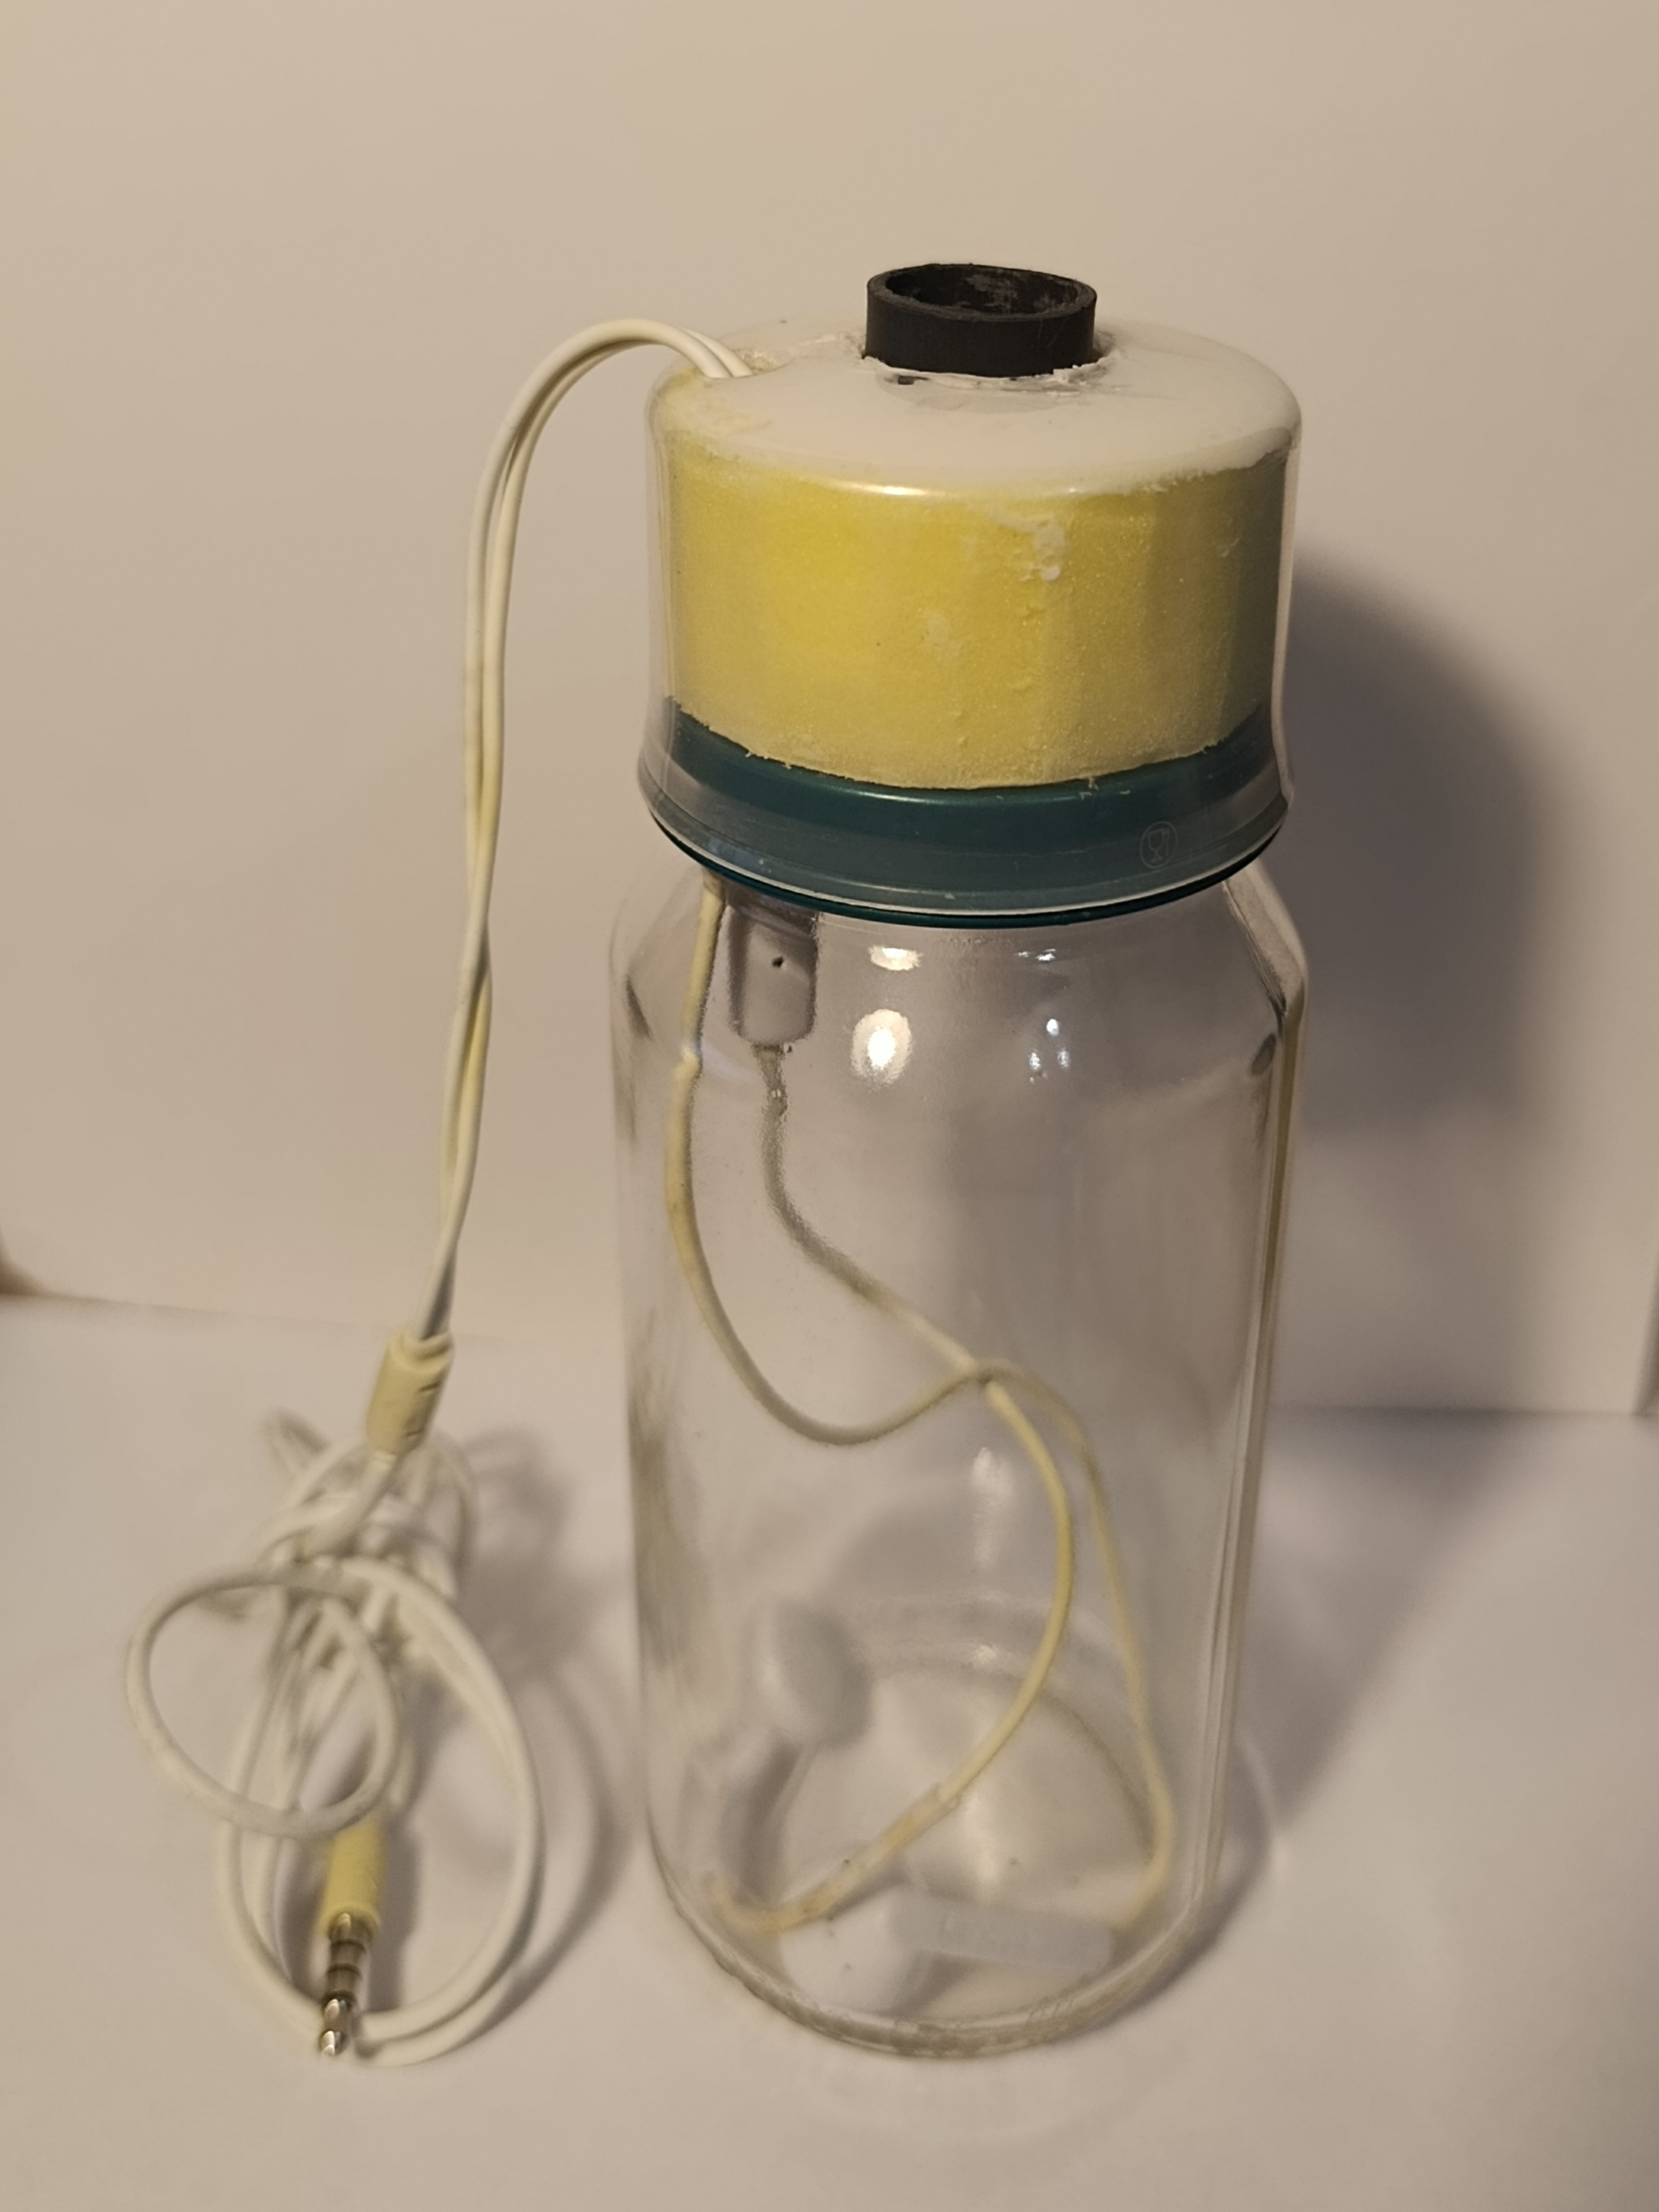
\includegraphics[width=\linewidth]{resonator}
			\caption{Общий вид собранного резонатора}
			\label{fig:real_setup}
		\end{subfigure}
		\hfill
		\begin{subfigure}[b]{0.63\linewidth}
			\centering
			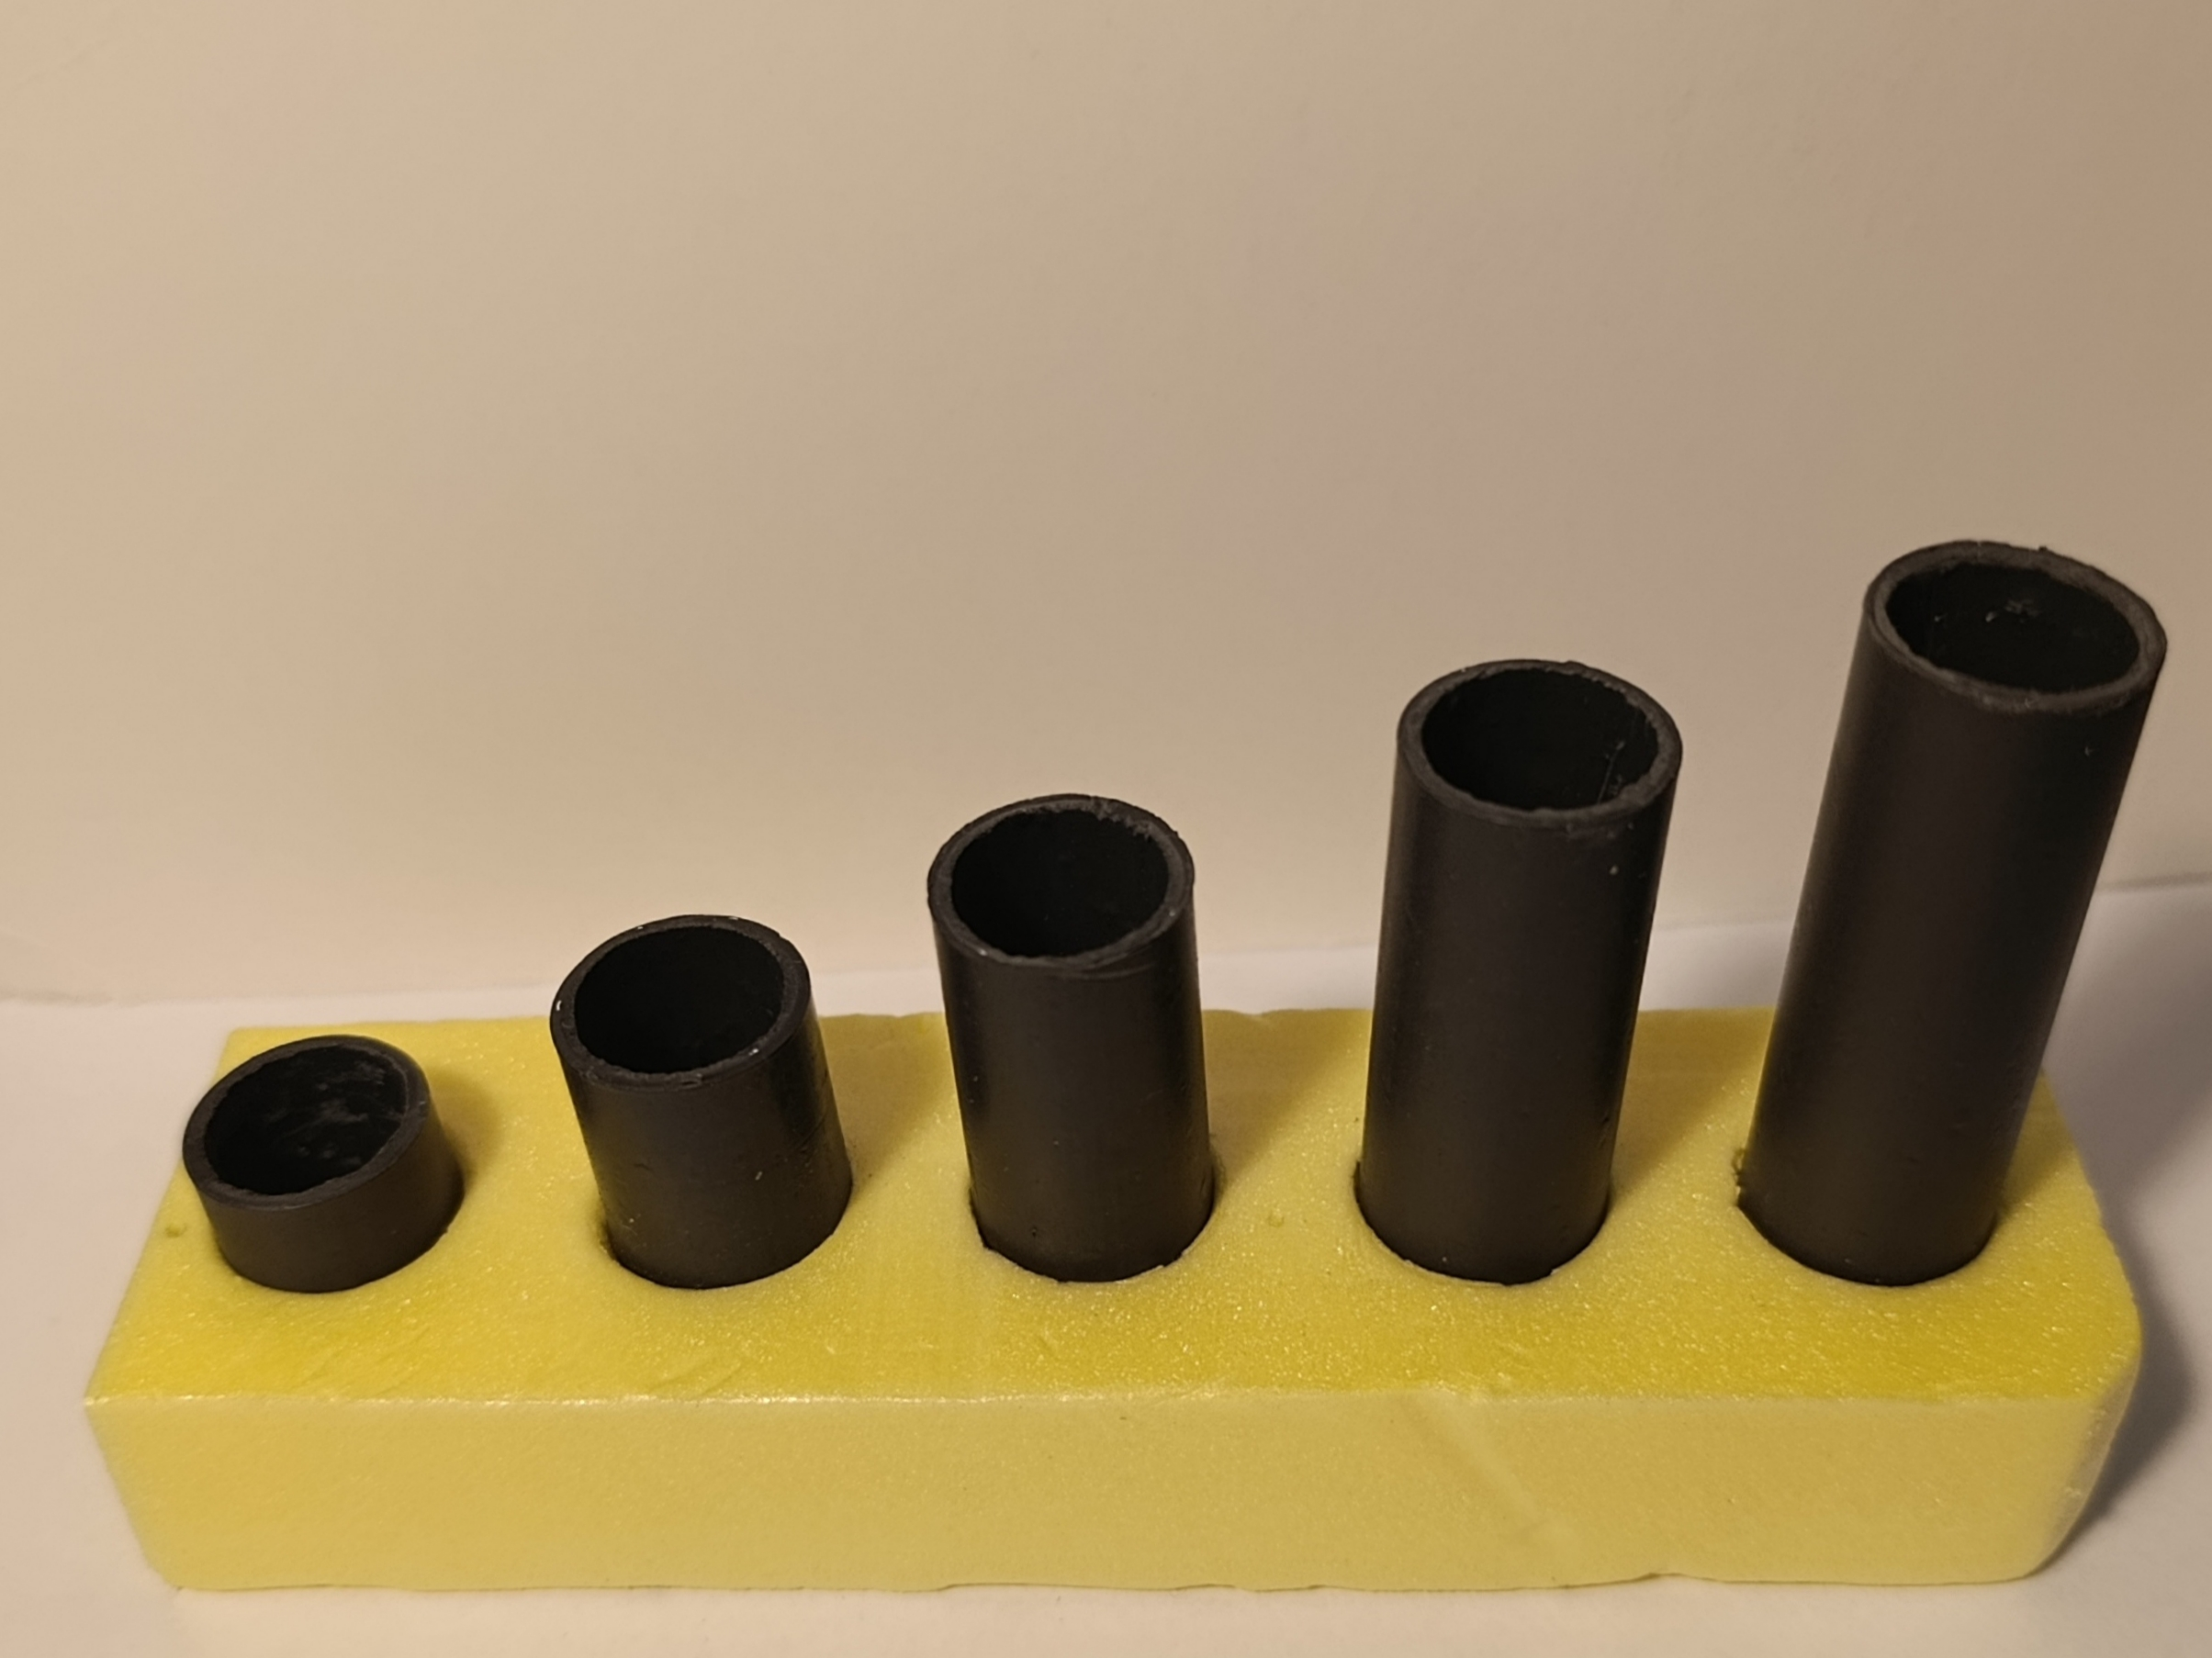
\includegraphics[width=\linewidth]{tubes}
			\caption{Набор добавочных трубок}
			\label{fig:additional_tubes}
		\end{subfigure}
		
		\caption{Экспериментальная установка}
		
	\end{figure}
	
	\section{Выбор сосуда}
	
	\hspace{4mm} В качестве резонатора мы использовали стеклянную банку с модифицированным горлышком. При выборе сосуда и изготовлении горлышка мы исходили из следующих требований:
	\begin{itemize}
		\item объём полости должен быть много больше объёма шейки;
		\item горлышко должно иметь цилиндрическую форму;
		\item края отверстия должны быть отчётливыми;
		\item стенки сосуда и горлышка должны быть жёсткими, чтобы их деформацией при тепловых и акустических воздействиях можно было пренебречь.
	\end{itemize}
	
	В исходной металлической крышке были сделаны отверстия для добавочных трубок и для провода  наушников. Сверху на металлическую крышку был положен слой пенопласта. На них плотно натягивалась внешняя пластиковая крышка. Все щели и отверстия были загерметизированы. Такая конструкция позволила получить достаточно жёсткий сосуд с устойчивой геометрией.
	
	
	
	\section{Добавочные трубки}
	
	\hspace{4mm} В первой серии эксперимента мы устанавливали в искусственно сформированное горлышко цилиндрические пластиковые трубки одного внутреннего диаметра и разной длины \(L\). Отверстия в металлической крышке и пенопласте были выполнены под диаметр этих трубок. При установке мы добивались плотной посадки и дополнительно герметизировали соединение так, чтобы воздух не проходил через щели вокруг трубки.
	
	К добавочным трубкам предъявлялись следующие требования:
	\begin{enumerate}
		\item внутренний диаметр должен быть одинаковым для всех трубок и совпадать с диаметром искусственного горлышка;
		\item форма поперечного сечения должна быть близка к круговой;
		\item стенки должны быть достаточно жёсткими;
		\item соединение с крышкой должно быть по возможности соосным;
		\item насадка не должна создавать щелей, резких уступов и заметных боковых утечек воздуха.
	\end{enumerate}
	
	
	В работе использовался набор пластиковых трубок разной длины и одного диаметра. Их длины и диаметр приведены далее в разделе с результатами предварительных измерений.
		
	
	\chapter{Методика эксперимента}
	
	\section{Измерение геометрических параметров}
	
	\hspace{4mm} Сначала предполагается определить:
	
	\begin{enumerate}
		\item объём банки \(V\);
		\item внутренний диаметр горлышка \(d\);
		\item длины всех добавочных трубок \(L_1,L_2,\dots\).
	\end{enumerate}
	
	Объём банки удобнее всего определять по разности масс пустой банки и заполненной водой. 
	
	
	\section{Определение резонансной частоты}
	
	\hspace{4mm} Для определения резонансной частоты сосуда следует построить его \textit{амплитудно-частотную характеристику} (АЧХ) - зависимость амплитуды звуковых колебаний от их частоты $A(f)$. 
	
	Под амплитудой обычно понимается \textit{амплитуда звукового давления} $P$ (в паскалях) - максимальное отклонение давления от атмосферного.
	
	На практике удобно измерять \textit{уровень звукового давления} $L$ (в децибелах). Он определён следующим образом:
	
	\begin{equation}
		L = 20 \cdot \log_{10}\left(\frac{P_{ск}}{P_{эт}}\right)
	\end{equation}
	
	где $P_{ск}$ - среднеквадратичное звуковое давление, $P_{эт} = 20$ мкПа - эталонное звуковое давление (порог слышимости).
	
	Уровень звукового давления не выражается через амплитуду явно, так как среднеквадратичное значение зависит от формы звуковой волны. Однако имеет место положительная связь этих параметров: так, например, для синусоиды $P = \sqrt{2}P_{ск}$. Поэтому положение пика АЧХ не зависит от выбора координат.
	
	Часто уровень звукового давления обозначают SPL. В частности, так подписана соответствующая ось на АЧХ в программе <<REW>> (пример на рис. \ref{fig:afc}).
	
	
	\begin{figure}[h!]
		\centering
		
\includegraphics[width=0.8\linewidth]{AFC}
		\caption{Амплитудно-частотная характеристика, построенная в ПО <<REW>>}
		\label{fig:afc}
		
	\end{figure}
	
	
	
	Для построения АЧХ необходим источник звука (динамик) с линейно изменяющейся во времени частотой и приёмник (микрофон) с возможностью измерения звукового давления. Источником переменного напряжения постоянной амплитуды с линейной частотной модуляцией и измерителем звукового давления выступает компьютер со звуковой картой и установленным ПО <<REW>>. Динамики и микрофон есть на проводных наушниках, которые подключаются к компьютеру и опускаются внутрь сосуда. 
		
		
	При измерениях положение наушников внутри банки старались сохранять неизменным, поскольку смещение источника и приёмника звука влияет на форму АЧХ и может менять высоту резонансного пика. 
	
	
	\section{Измерение температуры}
	
	\hspace{4mm} Во второй серии эксперимента мы изменяли температуру воздуха внутри банки. Перед каждым измерением частоты мы выдерживали установку до установления теплового равновесия и контролировали температуру воздуха в банке с помощью трёх датчиков температуры: на дне банки, в центральной части полости и в горлышке. После того, как показания датчиков на разных уровнях становились близкими, температурные датчики аккуратно извлекались из банки и снималась АЧХ.
	
	\begin{figure}[h!]
		\centering
		\begin{subfigure}{0.54\textwidth}
			\centering
			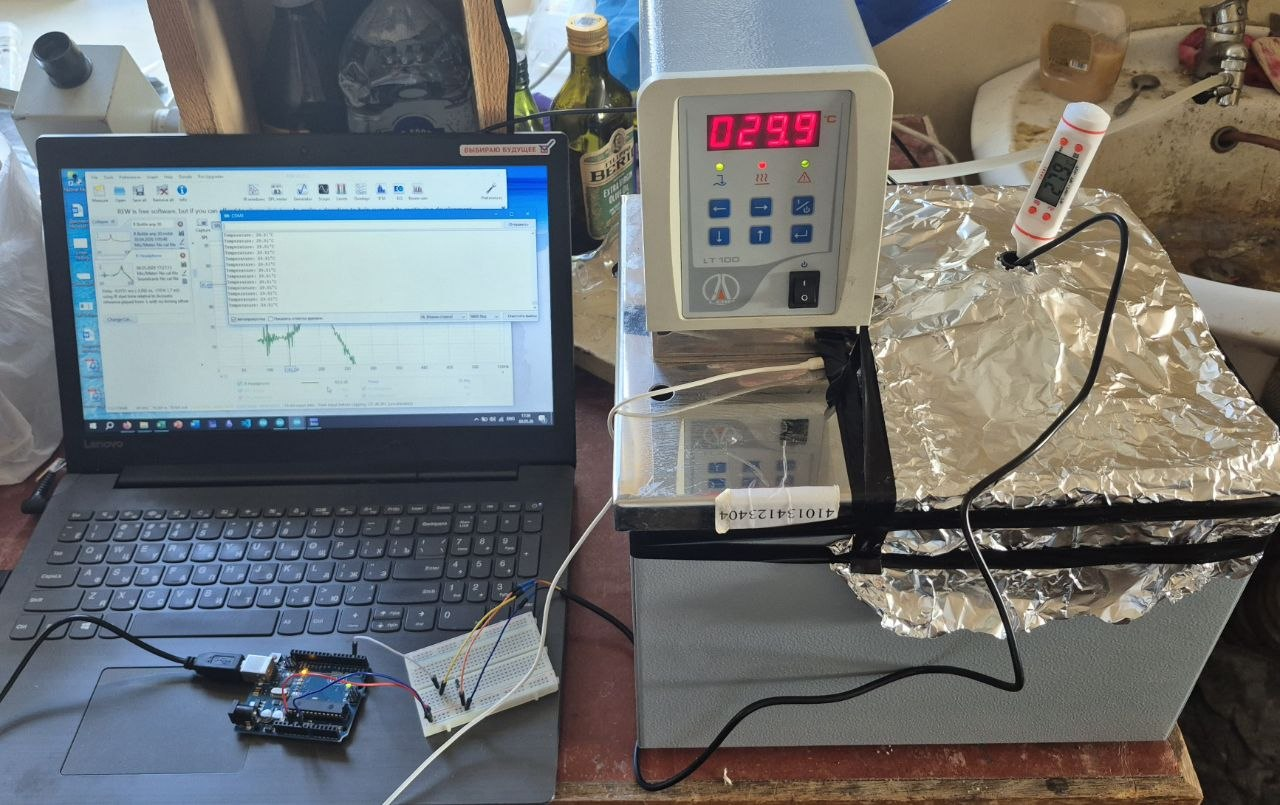
\includegraphics[width=\linewidth]{2 серия измерий.png}
			\caption{Общий вид установки при температурной серии.}
		\end{subfigure}
		\hfill
		\begin{subfigure}{0.45\textwidth}
			\centering
			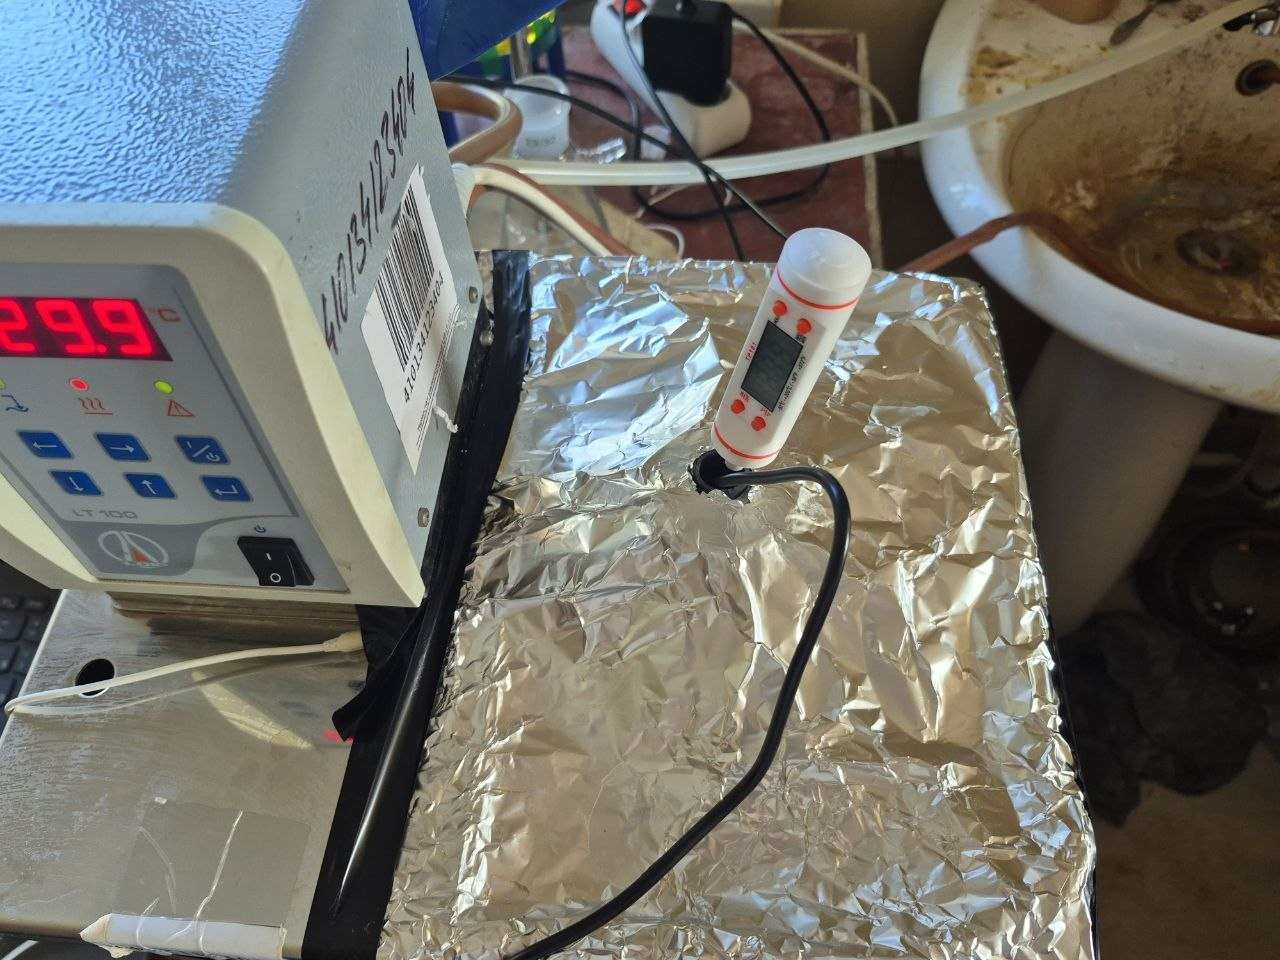
\includegraphics[width=\linewidth]{temperature_detail}
			\caption{Контроль температуры в термостате.}
		\end{subfigure}
		\caption{Измерение температуры воздуха в банке перед снятием резонансной частоты.}
		\label{fig:temperature_measurement_photo}
	\end{figure}
	
	Для поддержания нужной температуры использовался термостат. Банка помещалась в него, после чего сверху рабочая область закрывалась фольгой. В фольге оставлялось отверстие под добавочную трубку, чтобы геометрия горлышка во время измерений не изменялась (рис. \ref{fig:temperature_measurement_photo}).
	
	
	
	
	
	\section{Преимущества и ограничения метода}
	
	
	\hspace{4mm} Предлагаемый метод удобен тем, что:
	\begin{enumerate}
		\item использует простую и наглядную установку;
		\item позволяет связать акустический резонанс с термодинамической величиной \(\gamma\);
		\item включает собственную калибровку геометрического параметра;
		\item даёт два линейных графика, удобных для обработки;
		
	\end{enumerate}
	
	
	Вместе с тем метод основан на нескольких приближениях:
	\begin{enumerate}
		\item формула резонатора Гельмгольца предполагает, что шейка сравнительно короткая, а полость достаточно велика;
		\item газ рассматривается как идеальный;
		\item звуковой процесс считается адиабатическим;
		\item \(\gamma\) на рассматриваемом диапазоне температур принята постоянной.

	\end{enumerate}
	
	
	
	\chapter{Оценка погрешностей}
	
	\section{Определение резонансной частоты}
	
	\hspace{4mm} Из методики построения АЧХ следует, что погрешность возникает при воспроизведении звука нужной частоты и измерении амплитуды звуковых колебаний. Заметим, что при этом имеет место цифро-аналоговое и аналого-цифровое преобразование соответственно. Поэтому в обоих случаях источниками систематической погрешности выступают аппаратные ограничения звуковой карты и нелинейность АЧХ самих динамиков и микрофона (см. рис. \ref{fig:headphone-afc}).
	
	
	\begin{figure}[h!]
		\centering
		\includegraphics[width=0.8\linewidth]{"Headphone AFC"}
		\caption{АЧХ системы <<динамики - микрофон>> в диапазоне звукового восприятия (до 24 кГц)}
		\label{fig:headphone-afc}
	\end{figure}
	
	
	К счастью, измеренные резонансные частоты лежат в практически линейной области АЧХ (см. рис. \ref{fig:headphone-work-range}), поэтому её влияние можно не учитывать.
	
	
	\begin{figure}[h!]
		\centering
		\includegraphics[width=0.8\linewidth]{"Headphone work range"}
		\caption{Рабочий диапазон АЧХ системы <<динамики - микрофон>>}
		\label{fig:headphone-work-range}
	\end{figure}
	
	Теперь рассмотрим влияние аппаратных ограничений. Частота дискретизации звуковой карты используемого в работе компьютера составляет 48 кГц. При воспроизведении и записи частотно-модулированного звукового сигнала регистрируется 512 000 точек данных. Таким образом, разрешение составляет $\approx 0,09$ Гц.
	
	Источником случайной погрешности измерений выступают внешний шум и положение динамиков и микрофона в пространстве (распределение звукового поля внутри сосуда). Эта погрешность определена статистически многократным измерением резонансной частоты (см. рис. \ref{fig:many}). Среднеквадратичное отклонение составило $\sigma \approx 0,27$ Гц.
	
	\begin{figure}[h!]
		\centering
		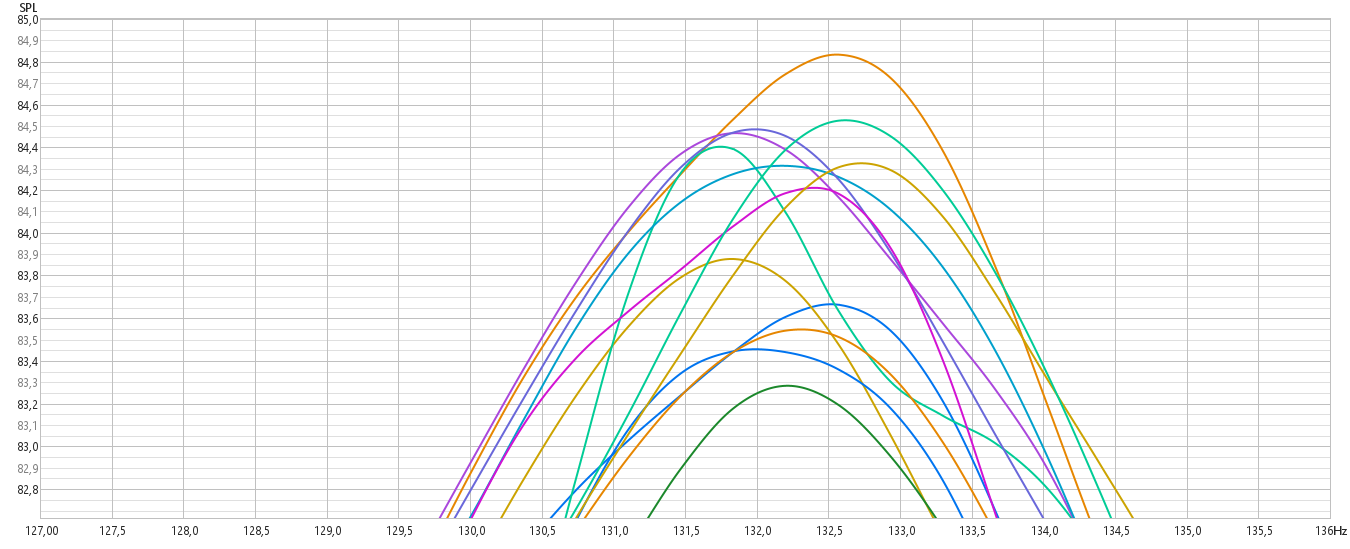
\includegraphics[width=\linewidth]{Many}
		\caption{Определение случайной погрешности резонансной частоты}
		\label{fig:many}
	\end{figure}
	
	
	
	
	
	
	
	
	\section{Погрешность эффективной длины шейки}
	
	\hspace{4mm} Если известны погрешности коэффициентов прямой \(a\) и \(b\), то относительная погрешность \(\delta\) при независимых ошибках оценивается по известной формуле:
	
	
	\begin{equation}
		\left(\frac{\sigma_\delta}{\delta}\right)^2
		=
		\left(\frac{\sigma_b}{b}\right)^2+
		\left(\frac{\sigma_a}{a}\right)^2
		\Rightarrow
		\sigma_\delta
		=
		\delta
		\sqrt{
			\left(\frac{\sigma_b}{b}\right)^2+
			\left(\frac{\sigma_a}{a}\right)^2
		}.
		\label{eq:sigma_delta}
	\end{equation}

	
	После нахождения \(\delta\) эффективная длина исходного горлышка вычисляется по формуле
	\begin{equation}
		L_{\text{эфф}}=L+\delta,
	\end{equation}
	где \(L\) --- геометрическая длина выбранной добавочной трубки.
	
	Если погрешности \(L\) и \(\delta\) независимы, то абсолютная погрешность эффективной длины определяется как
	\begin{equation}
		\sigma_{L_{\text{эфф}}}
		=
		\sqrt{
			\sigma_{L}^2+\sigma_\delta^2
		}.
		\label{eq:sigma_Leff}
	\end{equation}
	
	
	

	
	\section{Погрешность объёма бутылки}
	
	Объём банки \(V\) предполагается определять по массе воды, заполняющей полость:
	\[
	V=\frac{m}{\rho_{\text{воды}}} 
	\]
	и тогда погрешность объёма определяется в основном погрешностью измерения массы и, в меньшей степени, точностью учёта плотности воды.
	
	\section{Погрешность наклона графика \(f^2(T)\)}
	
	На втором этапе используется линейная зависимость
	\begin{equation}
		f^2(T)=
		\frac{\gamma R}{\mu}
		\frac{S}{4\pi^2 V L_{\text{эфф}}}
		\,T.
		\label{eq:err_f2T}
	\end{equation}
	
	Если аппроксимировать экспериментальные данные прямой
	\[
	f^2=kT+b,
	\]
	то в идеальной модели свободный член должен быть близок к нулю, а наклон \(k\) связан с \(\gamma\).
	
	Погрешность наклона \(\sigma_k\) определяется методом наименьших квадратов.
	
	
	\section{Итоговая погрешность \(\gamma\)}
	
	Из итоговой рабочей формулы следует, что \(\gamma\) зависит от четырёх основных экспериментальных величин:
	\[
	k,\qquad m,\qquad L_{\text{эфф}},\qquad d.
	\]
	
	Поскольку \(R\), \(\pi\) и \(\mu\) в данной работе считаются известными константами, относительная погрешность \(\gamma\) при независимых ошибках оценивается как
	
	\begin{equation}
		\left(\frac{\sigma_\gamma}{\gamma}\right)^2
		=
		\left(\frac{\sigma_k}{k}\right)^2+
		\left(\frac{\sigma_m}{m}\right)^2+
		\left(\frac{\sigma_{L_{\text{эфф}}}}{L_{\text{эфф}}}\right)^2+
		\left(2\frac{\sigma_d}{d}\right)^2.
		\label{eq:sigma_gamma_d}
	\end{equation}
	
	
	
	где
	
	\begin{multline}
				\left(\frac{\sigma_{L_{\text{эфф}}}}{L_{\text{эфф}}}\right)^2 = \left(\frac{\sqrt{\sigma_{L}^2+\sigma_\delta^2}}{L_{\text{эфф}}}\right)^2 = \left(\frac{\sigma_{L}}{L_{\text{эфф}}}\right)^2 + \left(\frac{\sigma_\delta}{L_{\text{эфф}}}\right)^2 =
				\left(\frac{\sigma_{L}}{L_{\text{эфф}}}\right)^2 + \left(\frac{\delta\sqrt{
						\left(\frac{\sigma_b}{b}\right)^2+
						\left(\frac{\sigma_a}{a}\right)^2}}{L_{\text{эфф}}}\right)^2 = \\ =	\left(\frac{\sigma_{L}}{L_{\text{эфф}}}\right)^2 + \left(\frac{\delta
						\sigma_b}{bL_{\text{эфф}}}\right)^2	+ \left(\frac{\delta
						\sigma_a}{aL_{\text{эфф}}}\right)^2	= \left(\frac{\sigma_{L}}{L_{\text{эфф}}}\right)^2 + \left(\frac{
						\sigma_b}{aL_{\text{эфф}}}\right)^2	+ \left(\frac{\delta
						\sigma_a}{aL_{\text{эфф}}}\right)^2
	\end{multline}
	
	Тогда абсолютная погрешность отношения теплоёмкостей равна
	\begin{equation}
	\boxed{\sigma_\gamma
		=
		\gamma
		\sqrt{
			\left(\frac{\sigma_k}{k}\right)^2+
			\left(\frac{\sigma_m}{m}\right)^2+
			 \left(\frac{\sigma_{L}}{L_{\text{эфф}}}\right)^2 + \left(\frac{
				\sigma_b}{aL_{\text{эфф}}}\right)^2	+ \left(\frac{\delta
				\sigma_a}{aL_{\text{эфф}}}\right)^2+
			4\left(\frac{\sigma_d}{d}\right)^2
	}}
	\label{eq:abs_sigma_gamma}
	\end{equation}
	
	\chapter{Результаты измерений}
	
	\section{Предварительные измерения}
	
	\hspace{4mm} Перед проведением основных серий эксперимента были измерены геометрические параметры резонатора и добавочных трубок. Масса воды, заполнившей банку, составила
	
	\begin{equation*}
		m = (278,7 \pm 0,1)\ \text{г}.
	\end{equation*}
	
	Длины нарезанных добавочных трубок представлены в таблице \ref{tab:L}.
	
	\begin{table}[h!]
		\centering
		\captionbox{Длины трубок}{
			\begin{tabular}{|r|ccccc|}
				\hline
				№        & 1        & 2        & 3        & 4        & 5         \\
				\hline
				$L$, мм    & 30,15    & 40,40    & 50,25    & 60,75    & 70,00 \\
				\hline
		\end{tabular}}
		\label{tab:L}
	\end{table}
	
	Было выполнено несколько измерений внутреннего диаметра в разных местах трубок.
	
	\begin{table}[h!]
		\centering
		\captionbox{Результаты измерения внутреннего диаметра трубок}{
			\begin{tabular}{|c|ccccccccc|}
				\hline
				№ измерения & 1 & 2 & 3 & 4 & 5 & 6 & 7 & 8 & 9 \\
				\hline
				$d$, мм & 14,00 & 14,10 & 13,60 & 13,75 & 13,80 & 14,20 & 14,15 & 14,25 & 13,75 \\
				\hline
				№ измерения & 10 & 11 & 12 & 13 & 14 & 15 & 16 & 17 & 18 \\
				\hline
				$d$, мм & 13,80 & 13,90 & 13,60 & 14,15 & 14,30 & 14,15 & 14,20 & 13,65 & 14,10 \\
				\hline
		\end{tabular}}
		\label{tab:diameter_measurements}
	\end{table}
	
	Среднее значение диаметра равно
	
	\begin{equation*}
		\overline d = \frac{1}{n}\sum_{i=1}^{n}d_i = 13,97\ \text{мм}.
	\end{equation*}
	
	Среднеквадратичный разброс отдельных измерений составил
	
	\begin{equation*}
		\sigma_d \approx 0,24\ \text{мм}.
	\end{equation*}
	
	В дальнейшем в расчётах использовалось значение
	
	\begin{equation*}
		\boxed{d = (14,0 \pm 0,2)\ \text{мм}.}
	\end{equation*}
	
	Здесь погрешность диаметра была взята не как погрешность среднего, а как среднеквадратичный разброс отдельных измерений. Это связано с тем, что разброс отражает не только случайную ошибку штангенциркуля, но и реальную неидеальность формы трубки.
	
	
	
	\section{Первая серия}
	
	\hspace{4mm} В первой серии эксперимента определялась концевая поправка \(\delta\) методом добавочных шеек. Для этого к искусственно сформированному горлышку последовательно присоединялись трубки разной длины \(L\), после чего для каждой трубки снималась амплитудно-частотная характеристика.
	
	Для каждой установленной трубки были сняты 5 АЧХ, после усреднения которых получена резонансная частота, соответствующая данной трубке (см. рис. \ref{fig:all-afc-1-bottle} и табл. \ref{tab:1-series}).
	
	\begin{figure}[h!]
		\centering
		\includegraphics[width=\linewidth]{"All necks"}
		\caption{Усреднённая по пяти измерениям АЧХ для каждой трубки}
		\label{fig:all-afc-1-bottle}
	\end{figure}
	
	\begin{table}[h!]
		\centering
		\captionbox{Результаты измерений в первой серии}{
			\begin{tabular}{|r|ccccc|}
				\hline
			L, мм	& 30,15    & 40,40    & 50,25    & 60,75    & 70,00 \\
				\hline
			f, Гц	& 198,7    & 183,3    & 168,4    & 157,6    & 148,3 \\
			\hline
			\end{tabular}}
		\label{tab:1-series}
	\end{table}
	
	По полученным данным построен график \(f^{-2}(L)\) с учётом погрешностей (см. рис. \ref{fig:graph1}). Найдены угловой коэффициент и свободный член уравнения аппроксимирующей прямой:
	
	\begin{equation*}
		a = (4,99 \pm 0,14) \cdot 10^{-7}\ \text{с}^2/\text{мм},
		\qquad
		b = (1,01 \pm 0,06) \cdot 10^{-5}\ \text{с}^2.
	\end{equation*}
	
	Получаем концевую поправку
	
	\begin{equation*}
		\boxed{\delta = \frac{b}{a} = (20,2 \pm 1,3)\ \text{мм}.}
	\end{equation*}
	
	\begin{figure}[h!]
		\centering
		\includegraphics[width=0.8\linewidth]{Neck length function}
		\caption{График зависимости \(f^{-2}(L)\)}
		\label{fig:graph1}
	\end{figure}
	
	Таким образом, первая серия эксперимента позволила определить концевую поправку, необходимую для расчёта эффективной длины горлышка во второй серии измерений.
	
	
	\section{Вторая серия}
	
	\hspace{4mm} Вторая часть эксперимента заключалась в снятии температурной зависимости резонансной частоты. Для этого строились АЧХ при пяти температурах в диапазоне \(30^\circ\text{C} \div 70^\circ\text{C}\) (см. рис. \ref{fig:temperature}). 
	
	\begin{table}[h!]
		\centering
		\captionbox{Результаты измерений во второй серии}{
			\begin{tabular}{|r|ccccc|}
				\hline
				$t$, \(^{\circ}\text{C}\) & 30 & 40 & 50 & 60 & 70 \\
				\hline
				$f$, Гц & 201,3 & 203,5 & 206,7 & 208,8 & 211,9 \\
				\hline
		\end{tabular}}
		\label{tab:2-series}
	\end{table}
	
	\begin{figure}[h!]
		\centering
		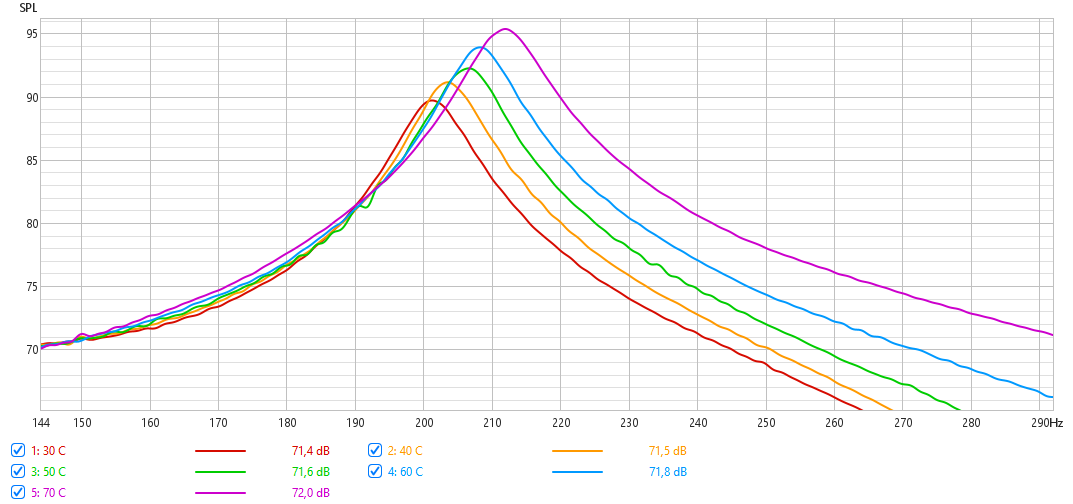
\includegraphics[width=1\linewidth]{All temperatures}
		\caption{Усреднённые по трём измерениям АЧХ сосуда при разных температурах}
		\label{fig:temperature}
	\end{figure}
	
	По этим точкам построен график \(f^2(t)\) (см. рис. \ref{fig:graph2}). Поскольку переход от температуры в градусах Цельсия к абсолютной температуре \(T=t+273,15\) не изменяет наклон линейной зависимости, для определения \(\gamma\) можно использовать угловой коэффициент графика \(f^2(t)\).
	
	\begin{figure}[h!]
		\centering
		\includegraphics[width=0.9\linewidth]{Temperature function}
		\caption{График зависимости \(f^2(t)\)}
		\label{fig:graph2}
	\end{figure}
	
	Угловой коэффициент был найден по методу наименьших квадратов:
	
	\begin{equation*}
		\boxed{k = (109 \pm 4)\ \text{Гц}^2/\text{К}.}
	\end{equation*}
	
	Во второй части опыта использовалась добавочная шейка под номером 1. Поэтому эффективная длина горла составила
	
	\begin{equation*}
		L_{\text{эфф}} = L_1 + \delta.
	\end{equation*}
	
	С учётом \(L_1 = 30,15\) мм и \(\delta = (20,2 \pm 1,3)\) мм получаем
	
	\begin{equation*}
		\boxed{L_{\text{эфф}} = (50,4 \pm 1,3)\ \text{мм}.}
	\end{equation*}
	
	
	
	\section{Нахождение $\gamma$}
	
	\hspace{4mm} По итоговой формуле \ref{eq:gamma_final} определим показатель адиабаты воздуха. Сначала вычислим произведение констант:
	
	\begin{equation*}
		\frac{16\pi\mu}{R}
		\approx
		\frac{16 \cdot 3,1416 \cdot 28,98\ \text{г}/\text{моль}}
		{8,314\ \text{Дж}/(\text{моль}\cdot \text{К})}
		\approx
		175,2\ \frac{\text{г}\cdot\text{К}}{\text{Дж}}
		=
		0,1752\ \frac{\text{с}^2\cdot\text{К}}{\text{м}^2}.
	\end{equation*}
	
	Теперь подставим измеренные величины:
	
	\begin{equation*}
		\dfrac{kVL_{\text{эфф}}}{d^2}
		=
		\frac{
			109\ \text{Гц}^2/\text{К}\cdot 0,2787\ \text{л}\cdot 50,4\ \text{мм}
		}{
			13,97^2\ \text{мм}^2
		}
		\approx
		7,85\ \frac{\text{Гц}^2\cdot \text{м}^2}{\text{К}}.
	\end{equation*}
	
	Тогда
	
	\begin{equation*}
		\gamma \approx 0,1752 \cdot 7,85 \approx 1,375.
	\end{equation*}
	
	Абсолютная погрешность равна
	
	\begin{equation*}
		\sigma_{\gamma}
		\approx
		1,375\cdot0,056
		\approx 0,08.
	\end{equation*}
	
	Получаем итоговое значение
	
	\begin{equation*}
		\boxed{\gamma = 1,38 \pm 0,08.}
	\end{equation*}
	
	
	
	\chapter{Анализ результатов}
	
	\hspace{4mm} В результате работы было получено значение показателя адиабаты воздуха
	
	\begin{equation*}
		\gamma = 1,38 \pm 0,08.
	\end{equation*}
	
	Табличное значение для воздуха при комнатных температурах близко к
	
	\begin{equation*}
		\gamma_{\text{табл}} \approx 1,40.
	\end{equation*}
	
	Полученный результат согласуется с табличным значением в пределах найденной погрешности. 
	
	
	Так как из формулы \ref{eq:gamma_final} следует зависимость
	
	\begin{equation*}
		\gamma \sim \frac{1}{d^2},
	\end{equation*}
	
	даже небольшое изменение диаметра заметно влияет на итоговый результат. Причина такого сильного влияния диаметра состоит в том, что в формулу резонатора Гельмгольца как один из основных геометрических параметров входит площадь сечения горлышка. При этом реальные пластиковые трубки не являются идеально цилиндрическими: их сечение немного отличается от кругового, и измеренный диаметр зависит от направления измерения. Поэтому в работе было корректно использовать не одно измерение диаметра, а среднее значение по серии измерений с оценкой разброса.
	
	Первая серия измерений показала линейную зависимость \(f^{-2}(L)\), что подтверждает применимость метода добавочных шеек. По этой зависимости была найдена концевая поправка
	
	\begin{equation*}
		\delta = (20,2 \pm 1,3)\ \text{мм}.
	\end{equation*}
	
	Полученное значение имеет правильный порядок величины: концевая поправка сравнима с диаметром горлышка, поскольку в колебательное движение вовлекается не только воздух внутри трубки, но и часть воздуха около её концов.
	
	Вторая серия измерений показала рост резонансной частоты с увеличением температуры. Это соответствует теоретической зависимости	$f^2 \sim T$. При нагревании воздуха скорость звука увеличивается, поэтому резонансная частота резонатора Гельмгольца также возрастает. Экспериментальные точки на графике \(f^2(t)\) достаточно хорошо ложатся на прямую, что подтверждает основную идею метода.
	
	Отдельно оценим применимость адиабатического приближения. Для этого сравним период акустических колебаний с характерным временем теплопроводности через радиус шейки. Радиус горлышка равен $r=d/2 \approx 7,0\ \text{мм}$.

	
	Для воздуха коэффициент температуропроводности имеет порядок
	
	\begin{equation*}
		\chi \approx 2,0\cdot10^{-5}\ \text{м}^2/\text{с}.
	\end{equation*}
	
	Характерное время теплопроводности можно оценить как
	
	\begin{equation*}
		\tau \sim \frac{r^2}{\chi}.
	\end{equation*}
	
	Подставляя \(r\), получаем
	
	\begin{equation*}
		\tau
		\sim
		\frac{(6,99\cdot10^{-3})^2}{2,0\cdot10^{-5}}
		\approx
		2,4\ \text{с}.
	\end{equation*}
	
	Период колебаний при частоте порядка \(200\) Гц равен
	
	\begin{equation*}
		T_{\text{кол}}=\frac{1}{f}\approx5\cdot10^{-3}\ \text{с}.
	\end{equation*}
	
	Следовательно,
	
	\begin{equation*}
		T_{\text{кол}}\ll \tau_T.
	\end{equation*}
	
	Это означает, что за один период колебаний тепло не успевает полностью передаться стенкам. Поэтому процесс сжатия и разрежения воздуха в резонаторе действительно можно считать близким к адиабатическому.
	
	Более точную оценку даёт толщина теплового пограничного слоя
	
	\begin{equation*}
		\delta_T=\sqrt{\frac{\chi}{\pi f}}.
	\end{equation*}
	
	При \(f\approx200\) Гц получаем
	
	\begin{equation*}
		\delta_T
		\approx
		\sqrt{\frac{2,0\cdot10^{-5}}{\pi\cdot200}}
		\approx
		1,8\cdot10^{-4}\ \text{м}
		=
		0,18\ \text{мм}.
	\end{equation*}
	
	Это значительно меньше радиуса горлышка. Значит, теплообмен со стенками происходит только в тонком слое около поверхности трубки и не должен приводить к полному переходу процесса к изотермическому режиму. Поэтому теплопроводность может влиять на добротность и давать малую систематическую поправку к частоте, но не является главным источником ошибки.
	
	Возможным дополнительным источником систематической погрешности является влажность воздуха. Водяной пар имеет показатель адиабаты и молярную массу, отличающиеся от соответствующих величин для сухого воздуха. В данной работе влажность напрямую не измерялась, поэтому её влияние не учитывалось в итоговой формуле. Однако при умеренной влажности этот эффект должен быть заметно меньше основной геометрической погрешности, связанной с определением диаметра.
	
	Также следует отметить влияние внутреннего расположения наушников, проводов и датчиков. Во время измерения частоты температурные датчики убирались из банки, чтобы не менять акустический объём и не искажать форму резонансного пика. При этом положение проводных наушников старались сохранять неизменным. Тем не менее распределение звукового поля внутри банки могло зависеть от положения источника и микрофона, что даёт вклад в случайную и систематическую погрешность определения резонансной частоты.
	
	Таким образом, основные источники неопределённости в работе связаны с:
	\begin{enumerate}
		\item определением внутреннего диаметра горлышка;
		\item нахождением эффективной длины по методу добавочных шеек;
		\item определением резонансной частоты по максимуму АЧХ;
		\item возможным температурным неравновесием между стенками, воздухом в полости и воздухом в горлышке;
		\item неучётом влажности воздуха.
	\end{enumerate}
	
	Наиболее существенным из этих факторов является геометрический: внутренний диаметр входит в итоговую формулу в квадрате, поэтому его уточнение оказалось принципиальным для получения правильного значения \(\gamma\).
	
	
	
	\chapter{Вывод}
	
	\hspace{4mm} В данной работе был реализован экспериментальный метод определения показателя адиабаты воздуха с помощью резонатора Гельмгольца. В качестве резонатора использовалась стеклянная банка с особым горлышком и набором добавочных трубок.
	
	Теоретической основой работы была формула резонатора Гельмгольца и выражение для скорости звука в идеальном газе.
	
	Из этих соотношений следует линейная зависимость \(f^2(T)\), позволяющая определить показатель адиабаты по угловому коэффициенту температурного графика.
	
	Эксперимент состоял из двух основных частей. В первой серии методом добавочных шеек была определена концевая поправка
	
	\begin{equation*}
		\delta = (20,2 \pm 1,3)\ \text{мм}.
	\end{equation*}
	
	Это позволило найти эффективную длину горлышка, использованную во второй серии:
	
	\begin{equation*}
		L_{\text{эфф}} = (50,4 \pm 1,3)\ \text{мм}.
	\end{equation*}
	
	Во второй серии была измерена зависимость резонансной частоты от температуры воздуха внутри банки. По графику \(f^2(t)\) был найден угловой коэффициент
	
	\begin{equation*}
		k = (109 \pm 4)\ \text{Гц}^2/\text{К}.
	\end{equation*}
	
	После измерения внутреннего диаметра трубок было получено
	
	\begin{equation*}
		d = (13,97 \pm 0,24)\ \text{мм}.
	\end{equation*}
	
	С учётом всех измеренных величин было найдено итоговое значение показателя адиабаты воздуха:
	
	\begin{equation*}
		\boxed{\gamma = 1,38 \pm 0,08.}
	\end{equation*}
	
	Полученный результат согласуется с табличным значением \(\gamma_{\text{табл}}\approx1,40\) в пределах экспериментальной погрешности.
	
	Таким образом, цель работы достигнута: была собрана экспериментальная установка, проведена калибровка эффективной длины горлышка, снята температурная зависимость резонансной частоты и по ней определён показатель адиабаты воздуха. Работа также показала, что для данного метода особенно важно аккуратно измерять внутренний диаметр горлышка, поскольку итоговое значение \(\gamma\) зависит от него как от \(1/d^2\).
	
	
\end{document}